\lecture{5}{7. April 2026}{Stability of Linear Feedback Systems}

\section{Stability of Linear Feedback Systems}

\subsection{Stability Definition}
Stability is often the most important concept in control systems.
A system might have a nice speed, accuracy, and disturbance rejection, but none of that matters if the system is unstable, because the output can then grow uncontrollably.

\begin{definition}[Stable System]
  A stable system is any system that gives a bounded output for any bounded input.
  This is also called \textit{BIBO}-stability (Bounded-Input, Bounded-Output).
  Stability is illustrated by the different cones on \Cref{fig:constab}.
\end{definition}

\begin{figure} [ht]
  \centering
  \begin{subfigure}[t]{0.3\textwidth}
    \centering
    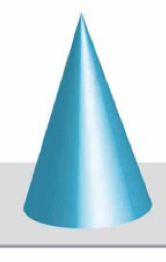
\includegraphics[height=1.8in]{./figures/constaba.png}
    \caption{Stable}
    \label{fig:constaba}
  \end{subfigure}
  \hfill
  \begin{subfigure}[t]{0.3\textwidth}
    \centering
    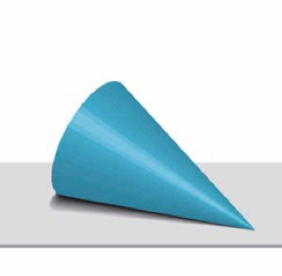
\includegraphics[height=1.8in]{./figures/constabb.png}
    \caption{Neutral}
    \label{fig:constabb}
  \end{subfigure}
  \hfill
  \begin{subfigure}[t]{0.3\textwidth}
    \centering
    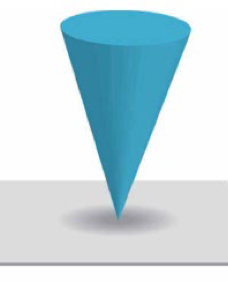
\includegraphics[height=1.8in]{./figures/constabc.png}
    \caption{Unstable}
    \label{fig:constabc}
  \end{subfigure}
  \caption{a cone in different configurations corresponding to a stable, neutral, and unstable system.}
  \label{fig:constab}
\end{figure}
On \Cref{fig:constab}, a cone is shown in three different configurations.
\Cref{fig:constaba} shows a cone standing on its base.
If you disturb it a little, it stays in a reasonable state (on its base).
Here, the system does not ``run away'' due to a small input.
On \Cref{fig:constabb} a cone lying on its side is shown.
Here, if you move it, it stays where you put it rather than returning or diverging (ideally).
This corresponds to marginal/neutral stability.
\Cref{fig:constabc} represents an unstable system by a cone balanced on its tip.
Here, any small disturbance makes the cone fall away.


\subsection{Stability Analysis with s-plane Approach}
On \Cref{fig:timeresps} a correlation between different pole locations and the corresponding time responses was shown.
This is summarized on \Cref{fig:polstab}.

\begin{figure} [ht]
  \centering
  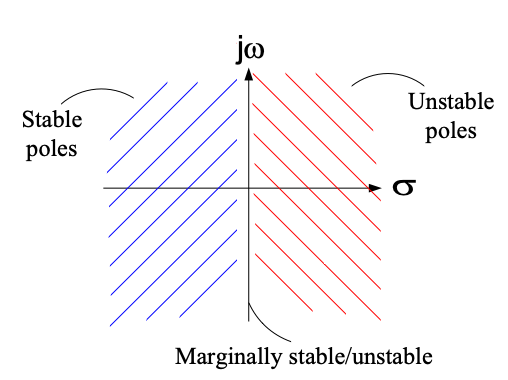
\includegraphics[width=0.5\linewidth]{./figures/polstab.png}
  \caption{Stability of poles depending on their location in the $s$-plane}
  \label{fig:polstab}
\end{figure}

Here, we see that a system is stable if all poles have negative real parts, and the system is unstable if any pole has positive real part.
Marginally stable systems are the special case, where poles are on the imaginary axis (real part equal to zero) and they are simple poles, while all other poles have negative real parts.
This happens, as a pole contributes a term like
\begin{equation*}
  e^{st} = e^{(\sigma + j\omega) t} = e^{\sigma t} e^{j \omega t}
\end{equation*}
so, if $\sigma < 0$, $e^{\sigma t}$ decays with time and vice versa.
For $\sigma = 0$, $e^{\sigma t} = 1$ so the response will have sustained oscillation with no decay or growth.

\subsubsection{Relative Stability of Feedback Control Systems}
Stability is rarely binary.
In general, we work with two different ideas: Absolute stability and relative stability.

Absolute stability is a simply yes/no question: ``Is the system stable or not?''.
If all poles are in the left half-plane, the system is absolutely stable.

Relative stability instead concerns itself with how stable a system is, how close the poles are to instability, and how oscillatory the response is.

These two concepts are compared on \Cref{fig:stabmar}.

\begin{figure} [ht]
  \centering
  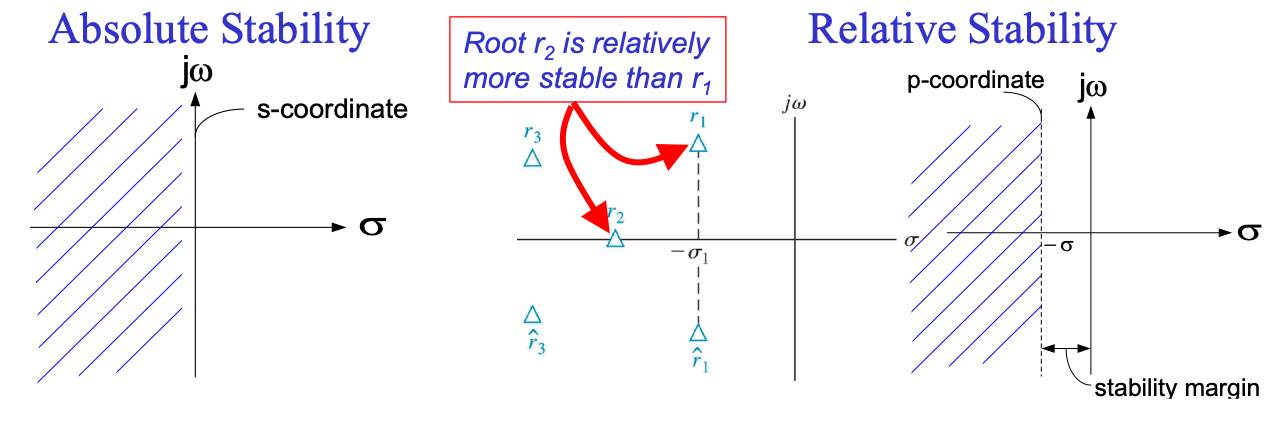
\includegraphics[width=0.8\linewidth]{./figures/stabmar.png}
  \caption{Comparison of different ideas of stability.}
  \label{fig:stabmar}
\end{figure}

On \Cref{fig:stabmar}, it is stated that $r_2$ is relatively more stable than $r_1$.
This is true, as $r_2$ is farther left in the $s$-plane, so its real part is more negative, meaning it is associated with a faster response decay.

The right figure on \Cref{fig:stabmar} shows a vertical line left of the imaginary axis.
The distance from that line to the imaginary axis is called the stability margin.
Here, we do not just want poles barely in the left half-plane.
We want them \textit{comfortably} to the left, so the system remains well-behaved even with modelling errors or parameter variations.

For complex poles, relative stability is also described by the damping ratio.
Higher damping ratios leads to less oscillation and better settling corresponding to  better relative stability. 


\subsection{Routh-Hurwitz Stability Criterion}
For a closed-loop LTI system, stability is determined by the roots of the characteristic polynomial
\begin{equation*}
  q(s) = a_n s^{n} + a_{n-1} s^{n-1} + \ldots  + a_1 s + a_0
\end{equation*}
these roots are the closed loop poles.

The Routh-Hurwitz method is a way to determine whether the roots of the characteristic equation have negative real parts just by looking at the coefficients of said equation.
Here, we use the Hurwitz's necessary condition stating that if $a_n > 0$, then for stability all coefficients must be positive.
This is only a necessary and not a sufficient condition.
I.e. a stable system will necessarily have positive coefficients to the characteristic equation, but having positive coefficients does not mean a system is necessarily stable.
This is exactly why Routh-Hurwitz is needed as it gives a stronger test.

\subsubsection{Routh Array}
To use the Routh-Hurwitz method, we start by building a so-called Routh array from the polynomial coefficients.
For
\begin{equation*}
  a_n s^{n} + a_{n-1} s^{n-1} + a_{n-2} s^{n-2} + \ldots  + a_0
.\end{equation*}
The Routh array is defined as:
\begin{equation*}
  \begin{array}{c|ccccc}
    s^{n} & a_n & a_{n-2} & a_{n-4}\\
  s^{n-1} & a_{n-1} & a_{n-3} & a_{n-5}\\
  s^{n-2} & b_{n-1} & b_{n-3} &b_{n-5} \\
  s^{n-3} & c_{n-1} & c_{n-3} & n_{n-5}\\
  \vdots  & \vdots  & \vdots  & \vdots \\
  s^{0} & h_{n-1} &  & \\
  \end{array}
\end{equation*}
where
\begin{align*}
  b_{n-1} &= \frac{a_{n-1} a_{n-2} - a_{n} a_{n-3}}{a_{n-1}} = - \frac{1}{a_{n-1}} \begin{vmatrix}
    a_n & a_{n-2}\\
  a_{n-1} & a_{n-3}\\
  \end{vmatrix} \\
  b_{n-3} &= - \frac{1}{a_{n-1}} \begin{vmatrix}
    a_n & a_{n-4}\\
  a_{n-1} & a_{n-5}\\
  \end{vmatrix} \\
    c_{n-1} &= - \frac{1}{b_{n-1}} \begin{vmatrix}
      a_{n-1} & a_{n-3}\\
    b_{n-1} & b_{n-3}\\
    \end{vmatrix}
.\end{align*}
I.e. the first two rows are arranged as $a_n, a_{n-2}, a_{n-4}$ and $a_{n-1, a_{n-3}}, a_{n-5}$, respectively and the next rows are then computed from the previous two.

The important result here, is then that the number of roots of $q(s)$ with positive real parts equals the number of sign changes in the first column of the Routh array.

\begin{exa}[Use of the Routh-Hurwitz Stability Criterion]
  We are given a characteristic polynomial in factored form as
  \begin{equation*}
    q(s) = \left( s - 1 + j \sqrt{7} \right) \left( s - 1 - j \sqrt{7} \right) \left( s + 3 \right)
  .\end{equation*}
  From this we see that the roots are $s = 1 + \pm j \sqrt{7}, -3$ so the first two have real part $1 > 0$, so two roots are in the right-half plane, meaning the system is unstable.
  Expanding the polynomial we get:
  \begin{equation*}
    q(s) = s^3 + s^2 + 2s + 24
  .\end{equation*}
  Here, all coefficients are positive, yet the system is still unstable, which directly proves the statement that the Hurwitz's necessary condition is not sufficient but only necessary.
  \tcblower
  For a cubic
  \begin{equation*}
    a_3 s^3 + a_2 s^2 + a_1 s + a_0
  \end{equation*}
  the Routh array is
  \begin{equation*}
    \begin{array}{c|ccc}
      s^3 & a_3 & a_1\\
    s^2 & a_2 & a_0\\
    s^{1} & b_1 & 0\\
    s^{0} & c_1 & 0\\
    \end{array}
  .\end{equation*}
  Here, $a_3 = 1, a_2 = 1, a_1 = 2, a_0 = 24$, so the first two rows are:
  \begin{equation*}
    \begin{array}{c|cc}
      s^3 & 1 & 2\\
    s^2 & 1 & 24\\
    \end{array}
  .\end{equation*}
  Now we compute
  \begin{equation*}
    b_1 = \frac{a_2 a_1 - a_3 a_0}{a_2} = \frac{1 \cdot 2 - 1\cdot 24}{1} = - 22
  \end{equation*}
  so the last row becomes
  \begin{equation*}
    c_1 = a_0 = 24
  \end{equation*}
  meaning the array is
  \begin{equation*}
    \begin{array}{c|ccc}
      s^3 & 1 & 2\\
    s^2 & 1 & 24\\
    s^{1} & -22 & 0\\
    s^{0} & 24 &0 \\
    \end{array}
  .\end{equation*}
  Here, there are two sign changes, so we have two 2 roots with positive real part meaning the system is unstable, which matches the expected result from the introduction. 
\end{exa}
